\documentclass[a4paper]{article}
\let\Tiny=\tiny
% Included packages ---------------------------------------------------------- %
\usepackage{inputenc}                 % utf-8 encoding, æ, ø , å, etc.
\usepackage{a4wide}                          % Adjust margins to better fit A4 format.
\usepackage{array}                           % Matrices.
\usepackage{amsmath}                         % Math symbols, and enhanced matrices.
\usepackage{amsfonts}                        % Math fonts.
\usepackage{amssymb}                         % Additional symbols.
\usepackage{wasysym}                         % More additional symbols.
\usepackage{mathrsfs}                        % Most additional symbols.
\usepackage[pdftex]{graphicx}                % Improved inclusion of .pdf-graphics files.
\usepackage{sidecap}                         % Floats with captions to the right/left.
\usepackage{cancel}                          % Visualize cancellations in equations.
\usepackage{enumerate}                       % Change counters (arabic, roman, etc.).
\usepackage{units}                           % Adds better looking fractions (nicefrac).
\usepackage{floatrow}                        % Multi-figure floats.
\usepackage{subfig}                          % Multi-figure floats.
\usepackage{caption}                         % Adds functionality to captions.
\usepackage{bm}                              % Bolded text in math mode.
\usepackage{combinedgraphics}                % Figures; let latex handle the text itself.
\usepackage[framemethod=default]{mdframed}   % Make boxes.
\usepackage{listings}                        % For including source code.
\usepackage[colorlinks]{hyperref}            % Interactive references, colored.
\usepackage{soul}                            % Make vertical bars through text.
\usepackage{nicefrac}                        % Nice fractions with \nicefrac.
\usepackage{mathtools}                       % Underbrackets, overbrackets.
\usepackage{wasysym}                         % \smiley{}-s!
\usepackage{multicol}                        % Multiple text columns.
\usepackage{capt-of}                         % Caption things which are not floats.
\usepackage[url=false]{biblatex}             % Citations (made easy).
\usepackage{simplewick}                      % Contractions using Wick's theorem for QFT.
\usepackage{booktabs}                        % Tables.
\usepackage{bbold}
\usepackage{tikz}

% Differentials -------------------------------------------------------------- %
\newcommand{\dt}{\,\mathrm{d}t}
\newcommand{\dx}{\,\mathrm{d}x}
\newcommand{\dr}{\,\mathrm{d}r}

% Derivatives ---------------------------------------------------------------- %
\newcommand{\der} [2]{\frac{\mathrm{d} #1}{\mathrm{d} #2}}   % Derivative.
\newcommand{\pder}[2]{\frac{\partial #1}{\partial #2}}       % Partial derivative.

% Matrices ------------------------------------------------------------------- %
\newcommand{\mat} [2]{\begin{matrix}[#1] #2 \end{matrix}}    % Nothing enclosing it.
\newcommand{\pmat}[2]{\begin{pmatrix}[#1] #2 \end{pmatrix}}  % Enclosing parentheses.
\newcommand{\bmat}[2]{\begin{bmatrix}[#1] #2 \end{bmatrix}}  % Enclosing square brackets.
\newcommand{\vmat}[2]{\begin{vmatrix}[#1] #2 \end{vmatrix}}  % Enclosing vertical bars.
\newcommand{\Vmat}[2]{\begin{Vmatrix}[#1] #2 \end{Vmatrix}}  % Enclosing double bars.

% Number sets ---------------------------------------------------------------- %
\newcommand{\R}{\mathbb{R}}
\newcommand{\Q}{\mathbb{Q}}
\newcommand{\N}{\mathbb{N}}
\newcommand{\Z}{\mathbb{Z}}
\newcommand{\C}{\mathbb{C}}

% Manually set alignment of rows / columns in matrices (mat, pmat, etc.) ----- %
\makeatletter
\renewcommand*\env@matrix[1][*\c@MaxMatrixCols c]{%
  \hskip -\arraycolsep
  \let\@ifnextchar\new@ifnextchar
  \array{#1}}
\makeatother

% References ----------------------------------------------------------------- %
\newcommand{\Fig}[1]{Fig.\ \ref{fig:#1}}
\newcommand{\fig}[1]{Fig.\ \ref{fig:#1}}
\newcommand{\eq} [1]{Eq.\ (\ref{eq:#1})}
\newcommand{\Eq} [1]{Eq.\ (\ref{eq:#1})}
\newcommand{\tab}[1]{Table \ref{tab:#1}}
\newcommand{\Tab}[1]{Table \ref{tab:#1}}

% Paragraph formatting ------------------------------------------------------- %
\setlength{\parindent}{5.5mm}
\setlength{\parskip}  {0mm}

% Source code listings ------------------------------------------------------- %
\definecolor{commentGreen}{RGB}{34,139,34}
\definecolor{keywordBlue}{RGB}{0,0,255}
\definecolor{stringPurple}{RGB}{160,32,240}
\lstset{language=matlab}
\lstset{basicstyle=\ttfamily\small}
\lstset{frame=single}
\lstset{stringstyle=\color{stringPurple}}
\lstset{keywordstyle=\color{keywordBlue}}
\lstset{commentstyle=\color{commentGreen}}
\lstset{morecomment=[l][\color{commentGreen}\bfseries]{\%\%}}
\lstset{showspaces=false}
\lstset{showstringspaces=false}
\lstset{showtabs=true}
\lstset{columns=fixed}
\lstset{breaklines}
\lstset{literate={~} {$\sim$}{1}}
\lstset{numbers=left}              
\lstset{stepnumber=1}
\renewcommand{\ttdefault}{pcr}
\lstdefinestyle{prt}{frame=none,basicstyle=\ttfamily\small}

% Convenient shorthand notation ---------------------------------------------- %
\newcommand{\nn}{\nonumber}
\newcommand{\e}[1]{\cdot10^{#1}}
\renewcommand{\i}{\hat{\imath}}
\renewcommand{\j}{\hat{\jmath}}
\renewcommand{\k}{\hat{k}}

% Caption position of tables at the top -------------------------------------- %
\floatsetup[table]{capposition=top}

% Black frame with white background ------------------------------------------ %
\newmdenv[linecolor=black,backgroundcolor=white]{exframe}

% Including vector drawings from inkscape ------------------------------------ %
\newenvironment{combFig}[5]{
  \begin{figure}[#1] 
    \centering 
    \includecombinedgraphics[vecscale=#2, keepaspectratio]{#3} 
    \caption{#4 \label{#5}}
  \end{figure}
  }

  {
}

% Including pdf graphics ----------------------------------------------------- %
\newenvironment{pdfFig}[5]{
  \begin{figure}[#1] 
    \centering 
    \includegraphics[width= #2]{#3} 
    \caption{#4 \label{#5}}
  \end{figure}
  }

  {
}

% Exercise and subexercise counters ------------------------------------------ %
\newcounter{excounter}
\renewcommand\theexcounter{\arabic{excounter}}
\newcommand\exlabel{\theexcounter}
\setcounter{excounter}{1}

\newcounter{subexcounter}
\renewcommand\thesubexcounter{\arabic{subexcounter}}
\newcommand\subexlabel{\thesubexcounter}
\setcounter{subexcounter}{1}

% Environments for exercises ------------------------------------------------- %
\newenvironment{exercise}[1]{
  \subsection*{Exercise \theexcounter: #1}
  \setcounter{subexcounter}{1}                      % Reset the subexercise counter to a.
  \addcontentsline{toc}{section}{\theexcounter: #1} % Add the exercise to TOC
  }
      % Exercise text.
  {
  \stepcounter{excounter}                           % Add one to the exercise counter.
  \newpage
}

% Environment for subexercises ----------------------------------------------- %
\newenvironment{subexercise}{
  \begin{exframe}
    \begin{itemize}  \setlength{\itemindent}{1cm}
      \item[{\bf Exercise \thesubexcounter}] 
	}
	  % Subexercise text.
	{
    \end{itemize}
  \end{exframe}
  \stepcounter{subexcounter}                        % Add one to the exercise counter.
}

% Environment for proofs ----------------------------------------------------- %
\newenvironment{proof}[2]{
  \begin{exframe}
    \begin{itemize}  \setlength{\itemindent}{0.6cm}
      \item[{\bf #1} {\bf #2}] 
	}
	  % Subexercise text.
	{
    \end{itemize}
  \end{exframe}
}

% Environment for answers ---------------------------------------------------- %
\newenvironment{answer}{}{}

% Set bibliography file and path for images.
\bibliography{references/fys4180ref.bib}
\graphicspath{{./images/}}
\newcommand{\includepdfgraphics}[2]{\includecombinedgraphics[#1]{./images/#2}}



\renewcommand{\L}{\hat{L}_z}
\renewcommand{\S}{\hat{S}_z}
\newcommand{\slater}{|P_1P_2\dots P_N\rangle}
\newcommand{\cm}{c_\mu}
\newcommand{\cn}{c_\nu}
\newcommand{\cmd}{c_\mu^\dagger}
\newcommand{\cnd}{c_\nu^\dagger}
\newcommand{\ca}{c_\alpha}
\newcommand{\cad}{c_\alpha^\dagger}
\newcommand{\cb}{c_\beta}
\newcommand{\cbd}{c_\beta^\dagger}

\renewcommand{\u}[1]{{\bf #1}_\uparrow}
\renewcommand{\d}[1]{{\bf #1}_\downarrow}

\newcommand{\boud}{b_{\u{1}}^\dagger}
\newcommand{\bou}{b_{\u{1}}}
\newcommand{\bodd}{b_{\d{1}}^\dagger}
\newcommand{\bod}{b_{\d{1}}}

\newcommand{\bfud}{b_{\u{5}}^\dagger}
\newcommand{\bfu}{b_{\u{5}}}
\newcommand{\bfdd}{b_{\d{5}}^\dagger}
\newcommand{\bfd}{b_{\d{5}}}

\newcommand{\ps}{{p\sigma}}
\newcommand{\cpp}{c_{p+}}
\newcommand{\cppd}{c_{p+}^\dagger}
\newcommand{\cpm}{c_{p-}}
\newcommand{\cpmd}{c_{p-}^\dagger}
\newcommand{\cqp}{c_{q+}}
\newcommand{\cqpd}{c_{q+}^\dagger}
\newcommand{\cqm}{c_{q-}}
\newcommand{\cqmd}{c_{q-}^\dagger}
\newcommand{\crp}{c_{r+}}
\newcommand{\crpd}{c_{r+}^\dagger}
\newcommand{\crm}{c_{r-}}
\newcommand{\crmd}{c_{r-}^\dagger}

% Title
\title{FYS-KJM4480 Project 2}
\date{}
\author{Morten Ledum}
% ---------------------------------------------------------------------------- %
% ---------------------------------------------------------------------------- %
\begin{document}
\maketitle
\subsection*{Exercise 1}

\begin{exframe}
We define first 
\begin{align}
\hat H = \hat H_0 + \hat V = \sum_{p\sigma} \epsilon_p c_\ps^\dagger c_\ps - \sum_{pq}\frac{1}{2}g \cpp^\dagger \cpm^\dagger \cqm \cqp,
\end{align}
with the ground state wave function of $\hat H_0$ being the Slater determinant (for the $N=4$ particles case) 
\begin{align}
|\Phi\rangle = c_{1+}^\dagger c_{1-}^\dagger c_{2+}^\dagger c_{2-}^\dagger |-\rangle.
\end{align}
The pair creation and annihilation operators are defined as follows
\begin{align}
\hat P^\dagger_p \equiv \cpp^\dagger \cpm^\dagger, \ \ \ \text{ and } \ \ \ \hat P_p \equiv \cpm \cpp,
\end{align}
with the number operator, the pair-number operator, and the spin-projection operators defined as
\begin{align}
\hat n_p \equiv \sum_\sigma c_\ps^\dagger c_\ps, \ \ \ \hat P \equiv \sum_p \hat P^\dagger_p \hat P_p, \ \ \ \text{ and } \ \ \ \hat S_z \equiv \frac{1}{2}\sum_\ps \sigma c_\ps^\dagger c_\ps.
\end{align}
\begin{itemize}
  \item[a)] Show that $\hat H_0$ and $\hat V$ commute with $\hat S_z$.
\end{itemize}
\end{exframe}
From the definitions of $\hat H_0$ and $\hat S_z$ we find that
\begin{align}
\hat H_0 \hat S_z &= \left(  \sum_\ps \epsilon_p c_\ps^\dagger c_\ps \right) \left(   \frac{1}{2}\sum_{p'\sigma'} \sigma' c_{p'\sigma'}^\dagger c_{p'\sigma'}  \right) \nn\\
%
&= \frac{1}{2}\sum_\ps \sum_{p'\sigma'}\sigma'  \epsilon_p c_\ps^\dagger c_\ps  c_{p'\sigma'}^\dagger c_{p'\sigma'} \nn\\
%
&= \frac{1}{2}\sum_\ps \sum_{p'\sigma'}\sigma'  \epsilon_p c_\ps^\dagger c_\ps  c_{p'\sigma'}^\dagger c_{p'\sigma'}.
\end{align}
Let us consider the operator string, and begin our long journey of anti-commuting things with
\begin{align}
c_\ps^\dagger c_\ps  c_{p'\sigma'}^\dagger c_{p'\sigma'} &= c_\ps^\dagger (-c_{p'\sigma'}^\dagger c_\ps   + \delta_{p\sigma p'\sigma'}) c_{p'\sigma'} \nn\\
%
&= c_{p'\sigma'}^\dagger c_\ps^\dagger  c_\ps c_{p'\sigma'}   + \delta_{p\sigma p'\sigma'}c_\ps^\dagger c_{p'\sigma'} \nn\\
%
&= -c_{p'\sigma'}^\dagger c_\ps^\dagger c_{p'\sigma'} c_\ps    + c_\ps^\dagger c_{p\sigma} \nn\\
%
&= -c_{p'\sigma'}^\dagger (- c_{p'\sigma'}c_\ps^\dagger + \delta_{p\sigma p'\sigma'}) c_\ps    + c_\ps^\dagger c_{p\sigma} \nn\\
%
&= c_{p'\sigma'}^\dagger c_{p'\sigma'}c_\ps^\dagger c_\ps -   \delta_{p\sigma p'\sigma'} c_{p'\sigma'}^\dagger c_\ps   + c_\ps^\dagger c_{p\sigma} \nn\\
%
&= c_{p'\sigma'}^\dagger c_{p'\sigma'}c_\ps^\dagger c_\ps -   c_{p\sigma}^\dagger c_\ps   + c_\ps^\dagger c_{p\sigma} \nn\\
%
&= c_{p'\sigma'}^\dagger c_{p'\sigma'}c_\ps^\dagger c_\ps,
\end{align}
where we have used the fundamental anti-commutation relations multiple times. We note that we have now switched the orders of $\hat H_0$ and $\hat S_z$, meaning that $\hat H_0 \hat S_z = \hat S_z \hat H_0$, i.e. the commutator vanishes.

We continue with $\hat V$ and $\hat S_z$, and find that
\begin{align}
\hat V \hat S_z &= \left(   - \sum_{pq}\frac{1}{2}g \cpp^\dagger \cpm^\dagger \cqm \cqp   \right)  \left(   \frac{1}{2}\sum_{p'\sigma'} \sigma' c_{p'\sigma'}^\dagger c_{p'\sigma'}  \right) \nn\\ 
%
&= -\frac{1}{4}\sum_{pq}\sum_{p'\sigma'}g\sigma' \cpp^\dagger \cpm^\dagger \cqm \cqp  c_{p'\sigma'}^\dagger c_{p'\sigma'},
\end{align}
from which we extract the operator string and compute
\begin{align}
\cpp^\dagger \cpm^\dagger \cqm \cqp  c_{p'\sigma'}^\dagger c_{p'\sigma'} &= \cpp^\dagger \cpm^\dagger \cqm (-  c_{p'\sigma'}^\dagger \cqp + \delta_{p'\sigma'q+}) c_{p'\sigma'} \nn\\
%
&= -\cpp^\dagger \cpm^\dagger  \cqm c_{p'\sigma'}^\dagger \cqp c_{p'\sigma'} + \cpp^\dagger \cpm^\dagger \cqm  \cqp \nn\\
%
&= -\cpp^\dagger \cpm^\dagger (- c_{p'\sigma'}^\dagger \cqm + \delta_{p'\sigma'q-}) \cqp c_{p'\sigma'} + \cpp^\dagger \cpm^\dagger \cqm  \cqp \nn\\
%
&= \cpp^\dagger \cpm^\dagger c_{p'\sigma'}^\dagger \cqm \cqp c_{p'\sigma'} - \delta_{p'\sigma'q-} \cpp^\dagger \cpm^\dagger \cqp c_{p'\sigma'}  + \cpp^\dagger \cpm^\dagger \cqm  \cqp \nn\\
%
&= c_{p'\sigma'}^\dagger \cpp^\dagger \cpm^\dagger \cqm \cqp c_{p'\sigma'} -  \cpp^\dagger \cpm^\dagger \cqp \cqm  + \cpp^\dagger \cpm^\dagger \cqm  \cqp \nn\\
%
&= c_{p'\sigma'}^\dagger \cpp^\dagger \cpm^\dagger c_{p'\sigma'} \cqm \cqp   + 2\cpp^\dagger \cpm^\dagger \cqm  \cqp \nn\\
%
&= c_{p'\sigma'}^\dagger \cpp^\dagger(-c_{p'\sigma'} \cpm^\dagger +\delta_{p'\sigma' p-}) \cqm \cqp   + 2\cpp^\dagger \cpm^\dagger \cqm  \cqp \nn\\
%
&= -c_{p'\sigma'}^\dagger \cpp^\dagger c_{p'\sigma'} \cpm^\dagger \cqm \cqp +\delta_{p'\sigma' p-} c_{p'\sigma'}^\dagger \cpp^\dagger \cqm \cqp  + 2\cpp^\dagger \cpm^\dagger \cqm  \cqp \nn\\
% 
&= -c_{p'\sigma'}^\dagger (- c_{p'\sigma'} \cpp^\dagger + \delta_{p'\sigma'p+}) \cpm^\dagger \cqm \cqp + \cpm^\dagger \cpp^\dagger \cqm \cqp  + 2\cpp^\dagger \cpm^\dagger \cqm  \cqp \nn\\
%
&= c_{p'\sigma'}^\dagger c_{p'\sigma'} \cpp^\dagger \cpm^\dagger \cqm \cqp - \delta_{p'\sigma'p+}c_{p'\sigma'}^\dagger \cpm^\dagger \cqm \cqp - \cpp^\dagger \cpm^\dagger  \cqm \cqp  + 2\cpp^\dagger \cpm^\dagger \cqm  \cqp \nn\\
%
&= c_{p'\sigma'}^\dagger c_{p'\sigma'} \cpp^\dagger \cpm^\dagger \cqm \cqp - \cpp^\dagger \cpm^\dagger \cqm \cqp + \cpp^\dagger \cpm^\dagger \cqm  \cqp \nn\\
%
&= c_{p'\sigma'}^\dagger c_{p'\sigma'} \cpp^\dagger \cpm^\dagger \cqm \cqp.
\end{align}
Fortunately, we note that we have again switched the order of the operators, meaning $[\hat V, \hat S_z]=0$ as expected.

\begin{exframe}
\begin{itemize}
  \item[b)] Show that $\hat H_0$ and $\hat V$ commute with $\hat P$.
\end{itemize}
\end{exframe}
Again, we simply insert the definitions and start anti-commuting operators past each other. Doing this yields
\begin{align}
 \hat P \hat H_0 &= \left(  \sum_p \hat P^\dagger_p \hat P_p\right) \left(  \sum_{p'\sigma'} \epsilon_{p'} c_{p'\sigma'}^\dagger c_{p'\sigma'} \right) \nn\\
%
&= \left(  \sum_p \cpp^\dagger \cpm^\dagger \cpm \cpp \right) \left(  \sum_{p'\sigma'} \epsilon_{p'} c_{p'\sigma'}^\dagger c_{p'\sigma'} \right)  \nn\\
%
&= \sum_p \sum_{p'\sigma'} \epsilon_{p'} \cpp^\dagger \cpm^\dagger \cpm \cpp   c_{p'\sigma'}^\dagger c_{p'\sigma'} \nn\\
%
&= -\sum_p \sum_{p'\sigma'} \epsilon_{p'} \cpp^\dagger \cpm^\dagger \cpp \cpm   c_{p'\sigma'}^\dagger c_{p'\sigma'},  \footnote{Note the minus sign (I had the wrong definitions of the $\hat P$ operator while typing this in, and didnt feel like redoing everything up to \eq{1} so I snuck in a sign change here).}
\end{align}
with
\begin{align}
\cpp^\dagger \cpm^\dagger \cpp \cpm c_{p'\sigma'}^\dagger c_{p'\sigma'} &= \cpp^\dagger \cpm^\dagger \cpp (-c_{p'\sigma'}^\dagger \cpm + \delta_{p'\sigma' p-}) c_{p'\sigma'} \nn\\
%
&= -\cpp^\dagger \cpm^\dagger \cpp c_{p'\sigma'}^\dagger \cpm c_{p'\sigma'}  + \delta_{p'\sigma' p-}  \cpp^\dagger \cpm^\dagger \cpp c_{p'\sigma'} \nn\\
%
&= -\cpp^\dagger \cpm^\dagger (-c_{p'\sigma'}^\dagger \cpp + \delta_{p'\sigma'p+}) \cpm c_{p'\sigma'}  +  \cpp^\dagger \cpm^\dagger \cpp \cpm \nn\\
%
&= \cpp^\dagger \cpm^\dagger c_{p'\sigma'}^\dagger \cpp \cpm c_{p'\sigma'}  - \delta_{p'\sigma'p+}\cpp^\dagger \cpm^\dagger \cpm c_{p'\sigma'}  +  \cpp^\dagger \cpm^\dagger \cpp \cpm \nn\\
%
&= c_{p'\sigma'}^\dagger \cpp^\dagger \cpm^\dagger \cpp \cpm c_{p'\sigma'}   - \cpp^\dagger \cpm^\dagger \cpm \cpp +  \cpp^\dagger \cpm^\dagger \cpp \cpm \nn\\
%
&= c_{p'\sigma'}^\dagger \cpp^\dagger \cpm^\dagger c_{p'\sigma'} \cpp \cpm    + \cpp^\dagger \cpm^\dagger \cpp \cpm  +  \cpp^\dagger \cpm^\dagger \cpp \cpm \nn\\
%
&= c_{p'\sigma'}^\dagger \cpp^\dagger \cpm^\dagger c_{p'\sigma'} \cpp \cpm    + \cpp^\dagger \cpm^\dagger \cpp \cpm  +  \cpp^\dagger \cpm^\dagger \cpp \cpm \nn\\
%
&= c_{p'\sigma'}^\dagger \cpp^\dagger (-c_{p'\sigma'}\cpm^\dagger + \delta_{p'\sigma'p-}) \cpp \cpm   +  2\cpp^\dagger \cpm^\dagger \cpp \cpm \nn\\
%
&= -c_{p'\sigma'}^\dagger \cpp^\dagger c_{p'\sigma'}\cpm^\dagger \cpp \cpm + \delta_{p'\sigma'p-} c_{p'\sigma'}^\dagger \cpp^\dagger  \cpp \cpm   +  2\cpp^\dagger \cpm^\dagger \cpp \cpm \nn\\
%
&= -c_{p'\sigma'}^\dagger (-c_{p'\sigma'}\cpp^\dagger +\delta_{p'\sigma'p+}) \cpm^\dagger \cpp \cpm + \cpm^\dagger \cpp^\dagger  \cpp \cpm   +  2\cpp^\dagger \cpm^\dagger \cpp \cpm \nn\\
%
&= c_{p'\sigma'}^\dagger c_{p'\sigma'}\cpp^\dagger \cpm^\dagger \cpp \cpm - \delta_{p'\sigma'p+} c_{p'\sigma'}^\dagger \cpm^\dagger \cpp \cpm - \cpp^\dagger\cpm^\dagger  \cpp \cpm   +  2\cpp^\dagger \cpm^\dagger \cpp \cpm \nn\\
%
&= c_{p'\sigma'}^\dagger c_{p'\sigma'}\cpp^\dagger \cpm^\dagger \cpp \cpm - \cpp^\dagger \cpm^\dagger \cpp \cpm  +  \cpp^\dagger \cpm^\dagger \cpp \cpm \nn\\
%
&= c_{p'\sigma'}^\dagger c_{p'\sigma'}\cpp^\dagger \cpm^\dagger \cpp \cpm. \label{eq:1}
\end{align}
As before, we note that we have switched the order of the operators and thus the commutator $[\hat H_0,\hat P]=0$.

%Moving on now, I grow bored with typing all of this in (and I assume no one is going to bother reading it in detail anyway), so we the following we use some tricks. The first of which is noting that for a general Slater determinant $|\Psi\rangle = c_{i\sigma_i}^\dagger c_{j\sigma_j}^\dagger c_{k\sigma_k}^\dagger \dots c_{j\sigma_j}^\dagger |-\rangle$, operating with $\hat V$ involves doing 
%\begin{align}
%\hat V |\Psi\rangle = \sum_{pq}-\frac{1}{2}g \cpp^\dagger \cpm^\dagger \cqm \cqp |\Psi\rangle.
%\end{align}
%We note that the only way to get a non-zero result from the terms in the sum is to demand that $p+$ and $p-$ \emph{are} in $|\Psi\rangle$, while $q+$ and $q-$ are \emph{not}. But this means that we annihilate and create one particle with spin projection $\sigma=+$ (the $c_{p+}^\dagger$ and $c_{q+}$ operators) and we annihilate and create one particle with spin projection $\sigma=-$ (the $c_{p-}^\dagger$ and $c_{q-}$ operators). Thus the total spin projection of $|\Phi\rangle$ does not change under $\hat V$, and so it does not matter if we apply $\hat S_z$ before or after $\hat V$. 

Moving on, we consider the $\hat V \hat P$, and find
\begin{align}
\hat V \hat P &= \left(  \sum_{pq} -\frac{1}{2}g \cppd \cpmd \cqm \cqp \right) \left( \sum_r \crpd \crmd \crm \crp \right) \nn\\
%
&= -\frac{1}{2}g\sum_{pq}\sum_r \cppd \cpmd \cqm \cqp \crpd \crmd \crm \crp,
\end{align}
with
\begin{align}
\cppd \cpmd \cqm \cqp \crpd \crmd \crm \crp &= \cppd \cpmd \cqm (-\crpd\cqp  + \delta_{r+q+}) \crmd \crm \crp \nn\\
%
&= -\cppd \cpmd \cqm\crpd\cqp \crmd \crm \crp +  (\delta_{r+q+}) \cppd \cpmd \cqm \crmd \crm \crp \nn\\
%
&= -\cppd \cpmd (-\crpd\cqm + \delta_{r+q-})\cqp \crmd \crm \crp + A \nn\\
%
&= \cppd \cpmd \crpd\cqm \cqp \crmd \crm \crp - (\delta_{r+q-})\cppd \cpmd \cqp \crmd \crm \crp + A \nn\\
%
&= \crpd \cppd \cpmd \cqm \cqp \crmd \crm \crp + B \nn\\
%
&= \crpd \cppd \cpmd \cqm (- \crmd\cqp + \delta_{r-q+}) \crm \crp + B \nn\\
%
&= -\crpd \cppd \cpmd \cqm \crmd\cqp \crm \crp + (\delta_{r-q+}) \crpd \cppd \cpmd \cqm \crm \crp   + B \nn\\
%
&= -\crpd \cppd \cpmd (- \crmd\cqm + \delta_{r-q-})\cqp \crm \crp + C \nn\\
%
&= \crpd \cppd \cpmd \crmd\cqm \cqp \crm \crp - (\delta_{r-q-})\crpd \cppd \cpmd \cqp \crm \crp+ C \nn\\
%
&= \crpd \cppd \cpmd \crmd\cqm \cqp \crm \crp + D \nn\\
%
&= \crpd \crmd \cppd \cpmd \crm \cqm \cqp  \crp + D \nn\\
%
&= \crpd \crmd \cppd (- \crm\cpmd + \delta_{r-p-}) \cqm \cqp  \crp + D \nn\\
%
&= -\crpd \crmd \cppd \crm\cpmd  \cqm \cqp  \crp + (\delta_{r-p-}) \crpd \crmd \cppd\cqm \cqp  \crp + D \nn
\end{align}
\begin{align}
&= -\crpd \crmd \cppd \crm\cpmd  \cqm \cqp  \crp + E \nn\\
%
&= -\crpd \crmd (- \crm\cppd + \delta_{r-p+}) \cpmd  \cqm \cqp  \crp + E \nn\\
%
&= \crpd \crmd \crm\cppd \cpmd  \cqm \cqp  \crp - (\delta_{r-p+})\crpd \crmd \cpmd  \cqm \cqp  \crp + E \nn\\
%
&= \crpd \crmd \crm\cppd \cpmd \crp \cqm \cqp   + F \nn\\
%
&= \crpd \crmd \crm\cppd (- \crp\cpmd +\delta_{r+p-}) \cqm \cqp   + F \nn\\
%
&= -\crpd \crmd \crm\cppd \crp\cpmd \cqm \cqp + (\delta_{r+p-})\crpd \crmd \crm\cppd \cqm \cqp    + F \nn\\
%
&= -\crpd \crmd \crm(- \crp\cppd + \delta_{r+p+})\cpmd \cqm \cqp + G \nn\\
%
&= \crpd \crmd \crm \crp\cppd \cpmd \cqm \cqp - (\delta_{r+p+})\crpd \crmd \crm \cpmd \cqm \cqp + G \nn\\
%
&= \crpd \crmd \crm \crp\cppd \cpmd \cqm \cqp + H,
\end{align}
with the constants $A$ through $G$ defined as 
\begin{align}
A &\equiv \phantom{A - }\,\,(\delta_{r+q+}) \cppd \cpmd \cqm \crmd \crm \crp, \\
B &\equiv A - (\delta_{r+q-})\cppd \cpmd \cqp \crmd \crm \crp, \\
C &\equiv B + (\delta_{r-q+}) \crpd \cppd \cpmd \cqm \crm \crp, \\
D &\equiv C - (\delta_{r-q-})\crpd \cppd \cpmd \cqp \crm \crp, \\
E &\equiv D + (\delta_{r-p-}) \crpd \crmd \cppd\cqm \cqp  \crp, \\
F &\equiv E - (\delta_{r-p+})\crpd \crmd \cpmd  \cqm \cqp  \crp, \\
G &\equiv F + (\delta_{r+p-})\crpd \crmd \crm\cppd \cqm \cqp, \ \ \text{and}\\
H &\equiv G - (\delta_{r+p+})\crpd \crmd \crm \cpmd \cqm \cqp.
\end{align}
Showing that $H$ vanishes (the first and second cancel the seventh and eight, and the third through the sixth cancel each other) is left as an exercise for the reader (because frankly I grow bored with this, and I doubt you will even more than glance at these equations). 

We note that this shows $\hat V \hat P=\hat P \hat V$ and thus the commutator vanishes.

\begin{exframe}
\begin{itemize}
  \item[c)] Show that $\hat P$ commutes with $\hat S_z$.
\end{itemize}
\end{exframe}
Once again, from the definitions, we find
\begin{align}
\hat P \hat S_z &= \left( \sum_r \crpd \crmd \crm \crp \right) \left( \frac{1}{2}\sum_\ps \sigma c_\ps^\dagger c_\ps  \right) \nn\\
%
&= \frac{1}{2}\sum_r \sum_\ps  \sigma \crpd \crmd \crm \crp  c_\ps^\dagger c_\ps,
\end{align}
with
\begin{align}
\crpd \crmd \crm \crp  c_\ps^\dagger c_\ps &= \crpd \crmd \crm (-c_\ps^\dagger \crp + \delta_{p\sigma r+}) c_\ps \nn\\
%
&= -\crpd \crmd \crm c_\ps^\dagger \crp c_\ps + \delta_{p\sigma r+} \crpd \crmd \crm c_\ps \nn\\
%
&= -\crpd \crmd (- c_\ps^\dagger \crm + \delta_{p\sigma r-})\crp c_\ps +  \crpd \crmd \crm \crp \nn\\
%
&= \crpd \crmd c_\ps^\dagger \crm \crp c_\ps -  \delta_{p\sigma r-}\crpd \crmd\crp c_\ps + \crpd \crmd \crm \crp \nn\\
%
&= c_\ps^\dagger\crpd \crmd  \crm \crp c_\ps -  \crpd \crmd\crp \crm - \crpd \crmd \crp\crm  \nn\\
%
&= c_\ps^\dagger\crpd \crmd c_\ps  \crm \crp  -  2\crpd \crmd \crp\crm  \nn\\
%
&= c_\ps^\dagger\crpd ( c_\ps \crmd + \delta_{p\sigma r-})  \crm \crp  -  2\crpd \crmd \crp\crm  \nn\\
%
&= -c_\ps^\dagger\crpd  c_\ps \crmd \crm \crp + \delta_{p\sigma r-}c_\ps^\dagger\crpd  \crm \crp -  2\crpd \crmd \crp\crm  \nn
\end{align}
\begin{align}
&= -c_\ps^\dagger (- c_\ps\crpd + \delta_{p\sigma r+}) \crmd \crm \crp + \crmd\crpd  \crm \crp -  2\crpd \crmd \crp\crm  \nn\\
%
&= c_\ps^\dagger c_\ps\crpd \crmd \crm \crp - \delta_{p\sigma r+} c_\ps^\dagger\crmd \crm \crp + \crpd\crmd   \crp\crm -  2\crpd \crmd \crp\crm  \nn\\
%
&= c_\ps^\dagger c_\ps\crpd \crmd \crm \crp -  \crpd\crmd \crm \crp - \crpd \crmd \crp\crm  \nn\\
%
&= c_\ps^\dagger c_\ps\crpd \crmd \crm \crp +  \crpd\crmd \crp\crm  - \crpd \crmd \crp\crm  \nn\\
%
&= c_\ps^\dagger c_\ps\crpd \crmd \crm \crp.
\end{align}
We note that we have switched the order of operators and found equality, meaning the commutator must again vanish.
\begin{exframe}
\begin{itemize}
  \item[d)] Show that $[\hat P_p, \hat P_q^\dagger] = \delta_{pq}(1-\hat n_q).$
\end{itemize}
\end{exframe}
For the last time now (thankfully!) we begin from the definitions and find that
\begin{align}
\hat P_p \hat P_q^\dagger &= \cpm \cpp \cqpd \cqmd \nn\\
%
&= \cpm (-\cqpd\cpp + \delta_{q+p+}) \cqmd \nn\\
%
&= -\cpm \cqpd\cpp \cqmd + \delta_{q+p+} \cpm\cqmd \nn\\
%
&= -(- \cqpd\cpm + \delta_{q+p-})\cpp \cqmd + \delta_{q+p+} \cpm\cqmd \nn\\
%
&= \cqpd\cpm \cpp \cqmd - \delta_{q+p-}\cpp \cqmd + \delta_{q+p+} \cpm\cqmd \nn\\
%
&= \cqpd\cpm (-\cqmd\cpp + \delta_{q-p+}) - \delta_{q+p-}\cpp \cqmd + \delta_{q+p+} \cpm\cqmd \nn\\
%
&= -\cqpd\cpm \cqmd\cpp + \delta_{q-p+}\cqpd\cpm - \delta_{q+p-}\cpp \cqmd + \delta_{q+p+} \cpm\cqmd \nn\\
%
&= -\cqpd(- \cqmd\cpm + \delta_{q-p-})\cpp + \delta_{q-p+}\cqpd\cpm - \delta_{q+p-}\cpp \cqmd + \delta_{q+p+} \cpm\cqmd \nn\\
%
&= \cqpd\cqmd\cpm \cpp - \delta_{q-p-} \cqpd\cpp+ \delta_{q-p+}\cqpd\cpm - \delta_{q+p-}\cpp \cqmd + \delta_{q+p+} \cpm\cqmd \nn\\
&= \hat P_q^\dagger \hat P_p - \delta_{q-p-} \cqpd\cpp+ \delta_{q-p+}\cqpd\cpm - \delta_{q+p-}\cpp \cqmd + \delta_{q+p+} \cpm\cqmd. \label{eq:2}
\end{align}
Let us in more detail consider the extra four terms which have appeared in \eq{2}:
\begin{align}
- \delta_{q-p-} \cqpd\cpp&+ \delta_{q-p+}\cqpd\cpm - \delta_{q+p-}\cpp \cqmd + \delta_{q+p+} \cpm\cqmd \nn\\
&= - \delta_{qp}\delta_{--} \cqpd\cpp+ \delta_{qp}\delta_{-+}\cqpd\cpm - \delta_{qp}\delta_{+-}\cpp \cqmd + \delta_{qp}\delta_{++} \cpm\cqmd \nn\\
%
&= - \delta_{qp} \cqpd\cpp+  \delta_{qp} \cpm\cqmd \nn\\
%
&= \delta_{qp}\left(\cpm\cqmd  -\cqpd\cpp \right)\nn\\
%
&= \delta_{qp}\left(-\cqmd\cpm + \delta_{p-q-}  -\cqpd\cpp \right)\nn\\
%
&= \delta_{qp}\left(-\cqmd\cpm + \delta_{pq}\delta_{--}  -\cqpd\cpp \right)\nn\\
%
&= \delta_{qp}\left(\delta_{pq} -\cqmd\cpm  -\cqpd\cpp \right) = \delta_{pq}\left(\delta_{pq} - \hat n_q\right) = \delta_{pq}\left(1 - \hat n_q\right),
\end{align}
where we have used that the internal delta function just evaluates to one after evaluating the outer one. We note from this that $\hat P_p \hat P_q^\dagger = \hat P_q^\dagger \hat P_p + \delta_{pq} (1 - \hat n_p) \Rightarrow [\hat P_p, \hat P_q^\dagger] = \delta_{pq}(1-\hat n_p)$. 

\begin{exframe}
\begin{itemize}
  \item[e)] Show that $\hat P|\Phi\rangle=2|\Phi\rangle$, and that $\hat S_z|\Phi\rangle = 0 |\Phi\rangle$.
\end{itemize}
\end{exframe}
Restricting ourselves to the subspace of the total Hilbert space in which $P=2$, we note that we can write any Slater determinant as $|\Phi\rangle = |r\bar r s\bar s\rangle$, with $1 \le r,\bar r, s, \bar s \le 4$. The label $r,s$ denotes the $r/s$-th single particle orbital with positive spin-projection, while $\bar r, \bar s$ denotes the $r/s$-th single particle orbital with negative spin-projection.

Operating from the left with $\hat P$ on $|\Phi\rangle$ yields 
\begin{align}
\hat P |\Phi\rangle &= \sum_{p} \hat P_p^\dagger \hat P_p |\Phi\rangle \nn\\
%
&= \sum_{p} \cppd\cpmd \cpm \cpp |\Phi\rangle \nn\\ 
%
&= \sum_{p} \cppd\cpmd \cpm \cpp |r\bar r s \bar s\rangle.
\end{align}
Since operating on the Slater determinant with $\hat P_q=\cqm\cqp$ on $|\Phi\rangle$ yields $0$ unless a pair of $q$ states are in the determinant. This means 
\begin{align}
\hat P |\Phi\rangle &= \sum_{p} \cppd\cpmd \cpm \cpp |r\bar r s \bar s\rangle \nn\\
%
&= \crpd\crmd \crm \crp |r\bar r s \bar s\rangle + c_{s+}^\dagger c_{s-}^\dagger c_{s-} c_{s+} |r\bar r s \bar s\rangle \nn\\
%
&= |r\bar r s \bar s\rangle + |r\bar r s \bar s\rangle = 2|r\bar r s \bar s\rangle.
\end{align}

Moving on, we consider the action of $\hat S_z$ on $|\Phi\rangle$ and find
\begin{align}
\hat S_z |\Phi\rangle &= \frac{1}{2}\sum_\ps \sigma c_{p\sigma}^\dagger c_{p\sigma} |r\bar r s \bar s\rangle \nn\\
%
&= \frac{(-1)}{2} c_{r-}^\dagger c_{r-} |r\bar r s \bar s\rangle + \frac{(+1)}{2} c_{r+}^\dagger c_{r+} |r\bar r s \bar s\rangle + \frac{(-1)}{2} c_{s-}^\dagger c_{s-} |r\bar r s \bar s\rangle + \frac{(+1)}{2} c_{s+}^\dagger c_{s+} |r\bar r s \bar s\rangle \nn\\
&= \frac{1}{2}\left(1-1+1-1\right)  |r\bar r s \bar s\rangle = 0,
\end{align}
where all other $\ps$ combinations in the sum give zero since the Slater does not contain any of those orbitals. 

\begin{exframe}
\begin{itemize}
  \item[f)] Explain why the following set of Slater determinants form a basis for the subspace of Hilbert space with $S_z=0$ and $P=2$:
  \begin{align}
  |p\bar p q\bar q\rangle = \hat P_p^\dagger \hat P_q^\dagger |-\rangle, \ \ \ 1\le p<q\le M.
  \end{align}
  Here, $\bar p$ indicates the state $p-$, while $p$ indicates the state with $p+$. Draw spin-orbital diagrams for $M=4$ and label properly. Draw all the basis states. What is the dimension of the subspace (for arbitrary $M$)?
\end{itemize}
\end{exframe}
\begin{figure}
\begin{center}
  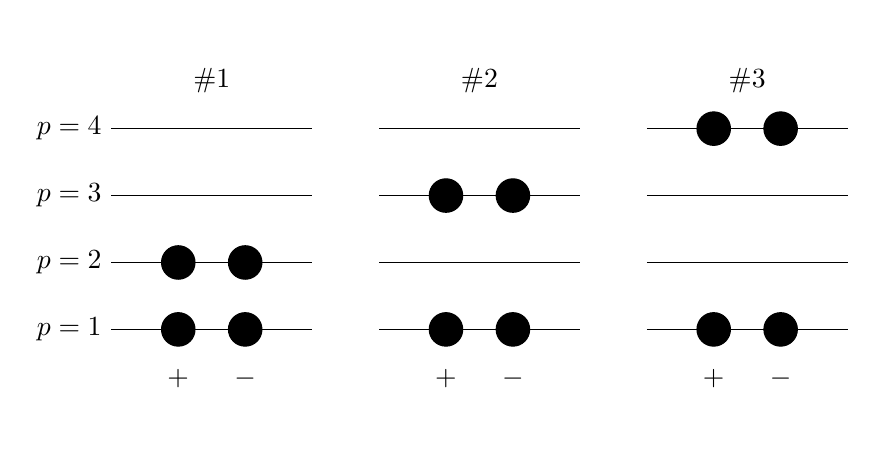
\begin{tikzpicture}[scale=0.85]
    \begin{scope}
      \foreach \i in {1,...,4}
      {
        \draw (-1,\i-1) node[anchor=east] {$p = \i$} --(2,\i-1);
      }
      \filldraw (0,0) node[anchor=north,inner sep=.5cm] {$+$} circle (0.25cm); 
      \filldraw (1,0) node[anchor=north,inner sep=.5cm] {$-$} circle (0.25cm);
      \filldraw (0,1) circle (0.25cm); 
      \filldraw (1,1) circle (0.25cm);
      \filldraw (0.5,4.5) node[anchor=north,inner sep=.5cm] {$\#1$} ; 
    \end{scope}
    \begin{scope}[xshift=4cm]
      \foreach \i in {1,...,4}
      {
        \draw (-1,\i-1) --(2,\i-1);
      }
      \filldraw (0,0) node[anchor=north,inner sep=.5cm] {$+$} circle (0.25cm); 
      \filldraw (1,0) node[anchor=north,inner sep=.5cm] {$-$} circle (0.25cm);
      \filldraw (0,2) circle (0.25cm); 
      \filldraw (1,2) circle (0.25cm);
      \filldraw (0.5,4.5) node[anchor=north,inner sep=.5cm] {$\#2$} ;
    \end{scope}
    \begin{scope}[xshift=8cm]
      \foreach \i in {1,...,4}
      {
        \draw (-1,\i-1) --(2,\i-1);
      }
      \filldraw (0,0) node[anchor=north,inner sep=.5cm] {$+$} circle (0.25cm); 
      \filldraw (1,0) node[anchor=north,inner sep=.5cm] {$-$} circle (0.25cm);
      \filldraw (0,3) circle (0.25cm); 
      \filldraw (1,3) circle (0.25cm);
      \filldraw (0.5,4.5) node[anchor=north,inner sep=.5cm] {$\#3$} ;
    \end{scope}
  \end{tikzpicture}
  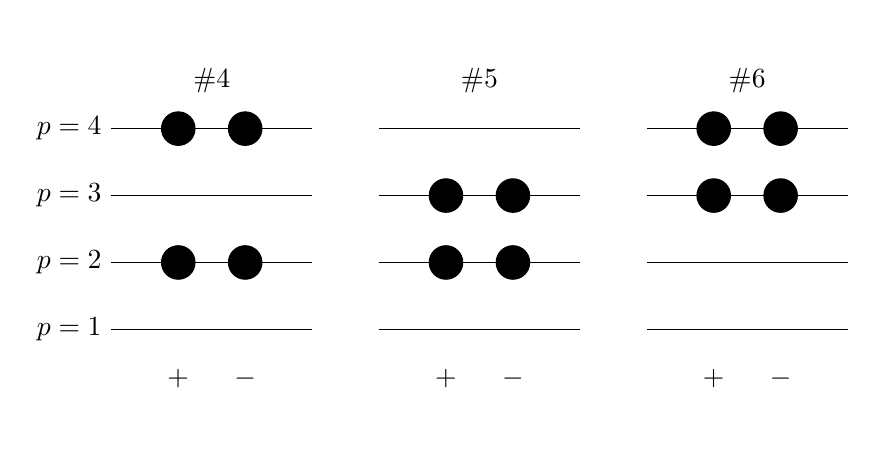
\begin{tikzpicture}[scale=0.85]
      \begin{scope}[xshift=0cm]
      \foreach \i in {1,...,4}
      {
        \draw (-1,\i-1) node[anchor=east] {$p = \i$} --(2,\i-1);
      }
      \filldraw (0,0) node[anchor=north,inner sep=.5cm] {$+$} ; 
      \filldraw (1,0) node[anchor=north,inner sep=.5cm] {$-$} ;
      \filldraw (0,1) circle (0.25cm); 
      \filldraw (1,1) circle (0.25cm); 
      \filldraw (0,3) circle (0.25cm); 
      \filldraw (1,3) circle (0.25cm);
      \filldraw (0.5,4.5) node[anchor=north,inner sep=.5cm] {$\#4$} ;
    \end{scope}
    \begin{scope}[xshift=4cm]
      \foreach \i in {1,...,4}
      {
        \draw (-1,\i-1) --(2,\i-1);
      }
      \filldraw (0,0) node[anchor=north,inner sep=.5cm] {$+$} ; 
      \filldraw (1,0) node[anchor=north,inner sep=.5cm] {$-$} ;
      \filldraw (0,1) circle (0.25cm); 
      \filldraw (1,1) circle (0.25cm); 
      \filldraw (0,2) circle (0.25cm); 
      \filldraw (1,2) circle (0.25cm);
      \filldraw (0.5,4.5) node[anchor=north,inner sep=.5cm] {$\#5$} ;
    \end{scope}
    \begin{scope}[xshift=8cm]
      \foreach \i in {1,...,4}
      {
        \draw (-1,\i-1) --(2,\i-1);
      }
      \filldraw (0,0) node[anchor=north,inner sep=.5cm] {$+$} ; 
      \filldraw (1,0) node[anchor=north,inner sep=.5cm] {$-$} ;
      \filldraw (0,3) circle (0.25cm); 
      \filldraw (1,3) circle (0.25cm); 
      \filldraw (0,2) circle (0.25cm); 
      \filldraw (1,2) circle (0.25cm);
      \filldraw (0.5,4.5) node[anchor=north,inner sep=.5cm] {$\#6$} ;
    \end{scope}
  \end{tikzpicture}
\end{center}
\caption{All the basis states in the subspace of the Hilbert space with $S_z=0$, $P=2$, $N=4$, and $M=4$. The states are arbitrarily assigned for all the states (except for the reference state which naturally is labeled with the index $1$). \label{fig:1}}
\end{figure}
Any state in the Hilbert space must have total spin zero, meaning that there must be an equal number of particles with positive spin-projection as there are with negative spin-projection. Also, we need the state to contain \emph{exactly} two pairs of particles in the $p-$ and $p+$ ($1\le p \le 4$) orbitals. Since the states represented in \fig{1} exhaust all possible states in the $M=N=4$ space under these constraints, we know that they form a basis for the space. Denoting these states by the numbers $I=1,2,\dots,6$, we note that they are orthogonal 
\begin{align}
\langle I | J \rangle &= \langle p\bar p q\bar q | r\bar r s\bar s\rangle = \delta_{pr}\delta_{\bar p \bar r}\delta_{qs}\delta_{\bar q \bar s}.
\end{align}

For $N=4$ with some $M\ge 2$, finding the number of total basis functions is a simple combinatorics problem. There are $M$ possible pair levels, and two pairs to place. The number of unique ways of distributing $2$ pairs across $M$ possible levels is $M$ choose $2$, i.e.
\begin{align}
\text{basis size} = {M\choose2} = \frac{M!}{2!(M-2)!}.
\end{align}
A few examples of the basis size are $M=4$: $6$, $M=10$: $45$, and $M=100$: $4950$. We note that in the general case, with no restrictions on $S_z$ and $P$, the entire Hilbert space will have 
\begin{align}
\text{basis size}_\text{general} = {2M\choose4},
\end{align}
e.g. $70$ for the $M=4$ case.

\begin{exframe}
\begin{itemize}
  \item[g)] Draw spin-orbital diagrams of the basis functions for the subspace $S_z=0$ and $P=0$, $M=4$. 
\end{itemize}
\end{exframe}
\begin{figure}
\begin{center}
  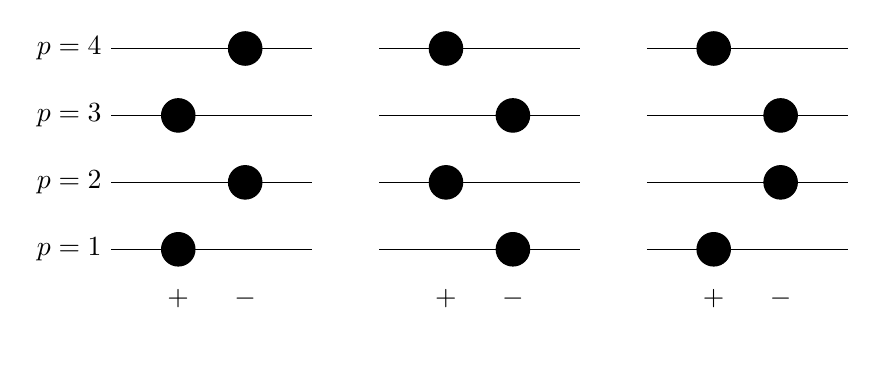
\begin{tikzpicture}[scale=0.85]
    \begin{scope}
      \foreach \i in {1,...,4}
      {
        \draw (-1,\i-1) node[anchor=east] {$p = \i$} --(2,\i-1);
      }
      \filldraw (0,0) node[anchor=north,inner sep=.5cm] {$+$} ; 
      \filldraw (1,0) node[anchor=north,inner sep=.5cm] {$-$} ;
      \filldraw (0,0) circle (0.25cm); 
      \filldraw (0,2) circle (0.25cm); 
      \filldraw (1,1) circle (0.25cm); 
      \filldraw (1,3) circle (0.25cm);
    \end{scope}
    \begin{scope}[xshift=4cm]
      \foreach \i in {1,...,4}
      {
        \draw (-1,\i-1) --(2,\i-1);
      }
      \filldraw (0,0) node[anchor=north,inner sep=.5cm] {$+$} ; 
      \filldraw (1,0) node[anchor=north,inner sep=.5cm] {$-$} ;
      \filldraw (0,1) circle (0.25cm); 
      \filldraw (0,3) circle (0.25cm); 
      \filldraw (1,0) circle (0.25cm); 
      \filldraw (1,2) circle (0.25cm);
    \end{scope}
    \begin{scope}[xshift=8cm]
      \foreach \i in {1,...,4}
      {
        \draw (-1,\i-1) --(2,\i-1);
      }
      \filldraw (0,0) node[anchor=north,inner sep=.5cm] {$+$} ; 
      \filldraw (1,0) node[anchor=north,inner sep=.5cm] {$-$} ;
      \filldraw (0,0) circle (0.25cm); 
      \filldraw (0,3) circle (0.25cm); 
      \filldraw (1,1) circle (0.25cm); 
      \filldraw (1,2) circle (0.25cm);
    \end{scope}
  \end{tikzpicture}
  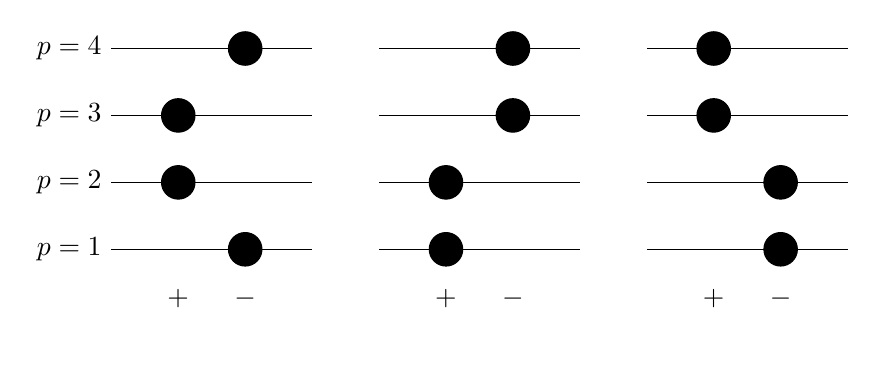
\begin{tikzpicture}[scale=0.85]
      \begin{scope}[xshift=0cm]
      \foreach \i in {1,...,4}
      {
        \draw (-1,\i-1) node[anchor=east] {$p = \i$} --(2,\i-1);
      }
      \filldraw (0,0) node[anchor=north,inner sep=.5cm] {$+$} ; 
      \filldraw (1,0) node[anchor=north,inner sep=.5cm] {$-$} ;
      \filldraw (1,0) circle (0.25cm); 
      \filldraw (1,3) circle (0.25cm); 
      \filldraw (0,1) circle (0.25cm); 
      \filldraw (0,2) circle (0.25cm);
    \end{scope}
    \begin{scope}[xshift=4cm]
      \foreach \i in {1,...,4}
      {
        \draw (-1,\i-1) --(2,\i-1);
      }
      \filldraw (0,0) node[anchor=north,inner sep=.5cm] {$+$} ; 
      \filldraw (1,0) node[anchor=north,inner sep=.5cm] {$-$} ;
      \filldraw (0,0) circle (0.25cm); 
      \filldraw (0,1) circle (0.25cm); 
      \filldraw (1,2) circle (0.25cm); 
      \filldraw (1,3) circle (0.25cm);
    \end{scope}
    \begin{scope}[xshift=8cm]
      \foreach \i in {1,...,4}
      {
        \draw (-1,\i-1) --(2,\i-1);
      }
      \filldraw (0,0) node[anchor=north,inner sep=.5cm] {$+$} ; 
      \filldraw (1,0) node[anchor=north,inner sep=.5cm] {$-$} ;
      \filldraw (1,0) circle (0.25cm); 
      \filldraw (1,1) circle (0.25cm); 
      \filldraw (0,2) circle (0.25cm); 
      \filldraw (0,3) circle (0.25cm);
    \end{scope}
  \end{tikzpicture}
\end{center}
\caption{All the basis states in the subspace of the Hilbert space with $S_z=0$, $P=0$, $N=4$, and $M=4$. \label{fig:2}}
\end{figure}
Assuming we are restricted to the $N=4$ case, we have the possible basis set shown in \fig{2}.


\begin{exframe}
\begin{itemize}
  \item[h)] Show that you can rewrite the Hamiltonian (with $\xi=1$) as 
  \begin{align}
  \hat H = \sum_p (p-1)\hat n_p - \frac{1}{2}g \left( \sum_p \hat P^\dagger_p \right) \left( \sum_q \hat P_q  \right).
  \end{align}
\end{itemize}
\end{exframe}
Inserting the definitions $\epsilon_p$ and $\hat V$ with $\hat P_p$ and $\hat P^\dagger_q$ we find
\begin{align}
\hat H &= \sum_\ps \epsilon_p c_\ps^\dagger c_\ps - \frac{1}{2}g \sum_{pq} \cppd \cpmd \cqm \cqp \nn\\
%
&= \sum_p (p-1) \left(\cppd \cpp + \cpmd \cpm \right) - \frac{1}{2}g \left(\sum_p\cppd \cpmd \right) \left( \sum_q \cqm \cqp \right) \nn\\
%
&= \sum_p (p-1) \hat n_p - \frac{1}{2}g \left(\sum_p\hat P_p^\dagger\right) \left( \sum_q \hat P_q\right).
\end{align}


\subsubsection{Exercise 2}
\begin{exframe}
\begin{itemize}
  \item[a)] Show that $\sum_s \hat P_s |p\bar p q \bar q\rangle = |p\bar p\rangle + |q \bar q\rangle$. Next, compute the closed form expression for all the matrix elements $\left\langle p'\bar p' q' \bar q' \right|\hat H \left|p\bar p q \bar q \right\rangle$.
\end{itemize}
\end{exframe}











\end{document}



% \begin{figure}[p!]
% \centering
% \includegraphics[width=12cm]{<fig>.pdf}
% \caption{\label{fig:1}}
% \end{figure}
 
% \lstinputlisting[firstline=1,lastline=2, float=p!, caption={}, label=lst:1]{<code>.m}

